\chapter{本研究における問題定義}
\label{issue}

\section{ボディビルにおけるポージングの重要性}
ポージングはトレーニングや減量と比べると練習時間が短く、相対的に重要度が下がってしまう傾向がある。
その原因としてはトレーニングの使用重量や減量における体重の変化のような定量的な指標がポージングには存在しないことが考えられる。
特に初心者では実際にステージで他の競技者と比較された経験が少ないため、ポージングの重要性を理解することが難しい。
また、ボディビルではトレーニングや、減量、日焼け、ポージングなどやることが多く、初心者は全てに時間やコストを払うのはとても大変である。
\section{ボディビルのポージングにおける悪いポージング}
ボディビルのポージングでは正解とされるポーズは存在しない。しかし、悪いポーズとされるポーズは存在する。
競技マニュアル\cite{JBBF2023}では悪いポーズの例として以下の図\ref{fig:badpose1},図\ref{fig:badpose2} が挙げられている。
図\ref{fig:badpose1}は片足を流していないことを指摘されていた。足を流すことでより足の筋肉のセパレーションやカットを強調できるため流していないことを指摘されていると考えられる。
図\ref{fig:badpose2}は腕をあげすぎていることを指摘されていた。腕をあげすぎてしまうと背中の広がりや上腕二頭筋などを強調することができないためこのような指摘がされたと考えられる。

  \begin{figure}[H]
    \begin{center}
        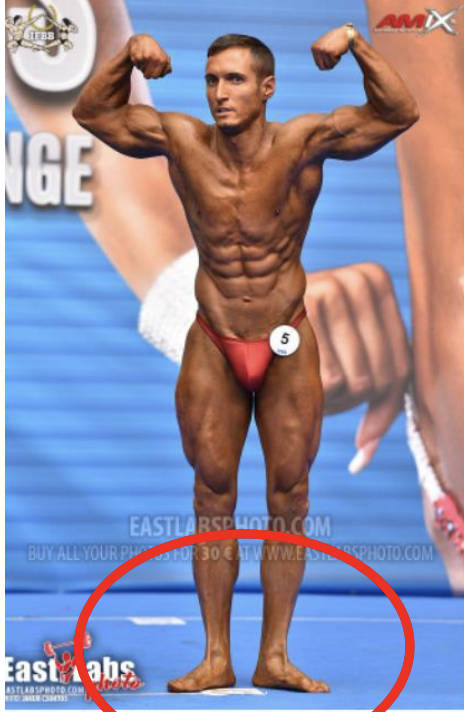
\includegraphics[width=7cm]{figures/badpose1.png}
        \caption{悪いポーズの例1}
        \label{fig:badpose1}
    \end{center}
  \end{figure}
  \begin{figure}[H]
    \begin{center}
        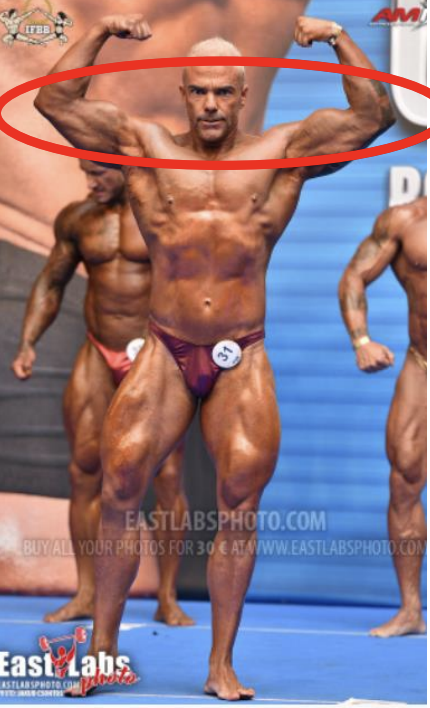
\includegraphics[width=7cm]{figures/badpose2.png}
        \caption{悪いポーズの例2}
        \label{fig:badpose2}
    \end{center}
  \end{figure}
\section{既存の練習方法における課題}
\subsection{鏡を用いた練習}
ボディビルのポージング練習では鏡の前でポーズを取り、視覚的に確認しながらポーズを修正していく方法が一般的である。しかし、初心者では鏡を使った練習ではどこを修正したら良いかわかりづらい。
また、鏡を見ながらの練習では左右反転している状態や、視点が自分と同じ高さにあることなどを理由に実際のステージ下にいる審査員とは異なる見え方をするため、本番を意識したポーズを獲得することが難しい。
一般的な家庭にあるサイズの鏡ではポーズをとった時に全身が映らなかったり、全身を俯瞰して見ることが難しかったりといった問題がある。
\subsection{動画や画像を使った練習}
写真や動画に撮る方法も鏡を使う練習と同じくよく行われる方法だ。カメラで撮影することで鏡と違い第三者視点でのポージングの確認ができることがメリットとして挙げられる。
第三者視点で見ることができるので、ポーズ全体を俯瞰して見ることや背中側のポーズを確認するといったことは可能になる。背中側のポーズは鏡では確認することが難しく、ポーズ習得の難易度が高いものになる。
しかしカメラで撮影する場合は、撮影のセッティングや撮影後の確認の手間がかかる。画像と比較してポーズを修正するには大きなディスプレイを利用するか、自身で覚えて鏡に映ったポーズと比較するといった方法が考えられるが、どちらも手間がかかる。
トップボディビルダーは毎トレーニング後にポージング練習を行うことを推奨していることが多いが、その度に撮影を行うのは鏡を使うことと比べ手軽とは言えない。
\subsection{他者からの指導}
上記2つの練習方法はどちらも1人で行う場合ではあるが、ポーズ改善のために他者からフィードバックを受ける方法もポーズを獲得するために重要な要素だ。
他者からの客観的な意見は自身のポーズを改善するのに役立つが、このアプローチにはいくつかの難点やデメリットがある。
例えば、専門のトレーナーや経験豊かな競技者からのフィードバックは有益だが、その指導を受けるためには高い費用がかかることが多い。
また、時間の都合を合わせる必要があり、特に初心者にとっては、頻繁な指導を受けることがハードルになることがある。さらに、自分に合った指導者を見つけること自体が難しい場合もあり、
地域によっては適切なトレーナーがいないこともある。これらのデメリットにもかかわらず、他者からのフィードバックはポーズ技術の向上に重要であり、適切なアドバイスを得るためにこれらの課題を乗り越える価値は大いにある。

\section{仮説}
上記の問題を踏まえ、本研究では次の仮説を検証する。
\begin{enumerate}
  \item 骨格推定用いた音声フィードバックを用いたポージング練習を行うことでポージングが改善される。
  \item 骨格推定用いた音声フィードバックを用いたポージング練習は鏡を用いたポージング練習と同等以上の効果を出すことができる。
  \item 骨格推定用いた音声フィードバックを用いたポージング練習は鏡を用いたポージング練習よりも効果を保持することができる。
\end{enumerate}
骨格推定を用いることで利用者のポーズを解析することができ、その計測結果を利用しフィードバックを行うことでリアルタイムでフィードバックを受けることができ
写真や動画撮影のようなポーズの中断をすることなくポーズ練習を行うことができる。また、単独でポーズ練習を行う際のデメリットであるフィードバックがない点を改善することができる。
そして音声を用いることで鏡を用いた練習のように視覚を制限することなくポーズの練習ができると考えられる。
また、音声フィードバックは鏡からの視覚情報よりも情報を受け取る頻度が少ないため、ガイダンス仮説におけるフィードバックの頻度による学習の保持の向上につながると考えられる。